\chapter{Related Work}

In this chapter, we will look at the state-of-the-art understanding of different topics presented in a variety of areas, which context relies on. These include techniques to annotate photos using image features, techniques to represent knowledge in ontologies, techniques to query data from a variety of sources.

\section{Photos and Annotation}

Kindberg \cite{kindberg2005ubiquitous} conducted a study on multiple subjects to analyze photo capture behavior. Specifically, they were trying to understand the different motivations for people to take photos. They found two main motivations -- \textit{affective} and \textit{functional}. A significant number of photos are captured to enrich a shared experience, or to share an experience with absent members like friends or family. Much lower, but a significant amount of photos were taken to share photos who were present at the event. Their study shows that photos are mostly used in social context, and lesser in personal context. Ames \cite{ames2007we} and Frohlich \cite{frohlich2002requirements} independently describe a survey conducted to study motivations for people to tag their photos. They noticed two broad motivations: Organization of photos and Communication with photos. Almost orthogonal to the applications observed by Kindberg, Ames and Frolich are brave new world applications for photography described in \cite{gemmell2002mylifebits, dumais2003stuff}, where life logs were collected in the form of photos, emails, document scans and stored in SQL Server database, and photos were retrieved using SQL queries. The photo content was tagged by the user in this case. The annotated photos are used exclusively for personal \textit{feedback} to improve quality of life. The medical advantages of collecting photos to log personal health are becoming very well known \cite{bell2010total}.

\subsection{Spatio-Temporal Annotation}
Ever since its release in 1995, EXIF metadata, contained in JPEG photos, has been exploited to organize pictures. Almost all photo management applications use timestamps to order photos in an album, a concept which has also been studied in academia \cite{graham2002time, hailpern2011youpivot}. Apple's iPhoto is the most common example of using both time and space to organize personal photos. Naaman et al.\ have exploited GPS attributes to extract place and person information \cite{naaman2005leveraging, naaman2005identity}. Rattenbury \cite{rattenbury2009methods} devised techniques to find tags which describe events or places by analyzing their spatiotemporal usage patterns. Sinha \cite{sinha2008concept} and Boutell \cite{boutell2005beyond} have used EXIF metadata to predict concepts such as (Indoor, Outdoor, Portrait, Landscape) to further organize these photos. Boll \cite{boll2007semantics} is a very interesting work which aggregates textual and experiential content from web 2.0 communities about places using a set of predefined rules. These works motivate the need for adding annotations to improve the overall experience of viewing a collection of photos.

\subsection{Computer Vision}

The Computer Vision community has contributed extensive work in the area of detecting scenes \cite{xiao2010sun}, humans \cite{dalal2005histograms} or geo localization \cite{hays2008im2gps}. Here we will specifically look at the part of the computer vision research which is relevant to face tagging.

\textbf{Face Recognition}
The face recognition problem is one of the primary problems taken on by the computer vision community, the others being action, pose, gesture recognition and human detection. One of the earliest works on recognizing people in faces was attempted by Turk and Pentland in \cite{turk1991eigenfaces}. The essence of the technique put forward here was to extract useful features which can be represented mathematically and compared using some distance measures (such as euclidean, mahalanobis or cosine distance) to features in an image database. This contribution sparked a large interest in the community to find more meaningful and powerful features, which led to Fisherfaces \cite{belhumeur1997eigenfaces} and more recently, local binary pattern \cite{ahonen2006face} features. SIFT features have also been used to identify faces \cite{bicego2006use, geng2009sift, luo2007person}. One of the big difficulties of such feature-based representation is the scalability of the technique. It is now well known that with the increasing number of candidates, these distance based techniques provide in lower performance \cite{wu2004probability}. A quick alternative is to increase the dimensions in the features to allow for more diversity, but it has been proven that as the number of dimensions increase, the maximum distance between the two points reduces, and if the number of dimensions is as less as 32, the distance is almost negligible \cite{beyer1999nearest}. Effectively, for dimensions more than 32, the distance between all points can be considered very small, and the concept of `nearest-neighbour' loses its meaning. Thus, an pure feature based technique cannot be used to build large scale real world photo tagging frameworks.

\textbf{Face Verification}
More recently, face verification techniques have attracted a lot of attention in the computer vision community. One of the earliest efforts towards robust face verification was undertaken by Huang et al.\ in \cite{huang2007labeled}. They constructed and annotated a dataset of profile photos of celebrities taken in unrestricted environments. Previous datasets such as FRGC \cite{phillips2005overview}, BioID \cite{jesorsky2001robust} and the color FERET database \cite{phillips1998feret} were criticized to have photos taken at very constrained environments thereby reducing the complexity of the face tagging problem. But the techniques which worked on such photos could not duplicate their performance in real-world photos. Huang's database, commonly known as the \textit{Faces In the Wild} has allowed many researchers to implement various face verification technologies. A recent and important development on top of Huang's work is that of Neeraj Kumar et al.\ \cite{nk_attribute_classifiers}, where the confidence of presence or absence of facial attributes such as range, skin color, hair style, gender, eye color features are used to train various classifiers to ultimately test if two given faces are of the same person or not? The technique was able to achieve up to 85.29\% accuracy on the LFW dataset. More recently, Berg \cite{berg2012tom} increased this accuracy to 93\% by automatically finding distinguishing features.

The interesting perspective face verification brings forward is in its contract with co-existing components in a system. Whereas, face recognition works as a standalone component, face verification doesn't make this assumption, and allows external components to filter candidates. This systemic behavior of face verification will prove to be very useful in future systems.

\textbf{Probabilistic Techniques}
Both face verification and recognition techniques seen so far assume that none of the input photos contain any annotation. But what if this assumption could be relaxed? A large number of photos on Facebook, Flickr or Google+ are annotated. If we further assume that these partial annotations are mostly true, the label propagation technique by Cao et al.\ \cite{cao2008annotating} can be applied to annotate the rest of the dataset. This technique was tested on propagating concept based tags (such as beach, fun, dinner, yard) on personal photo datasets. Also, Barthelmess et al.\ extract semantic tags from noisy datasets containing discussions, speeches about a set of photos in question\cite{barthelmess2007toward}. 

\textbf{Miscellaneous Techniques}
Collaborative games also have been evaluated as a possible way to tag photos\cite{diakopoulos2007photoplay}. Systems like Picasa, iPhoto and \cite{graham2002time} organize photos based on time, GPS coordinates and sometimes faces in the photo. These attributes of the photo do not capture event semantics \cite{sawant2011automatic}. Events are a natural way of categorizing photo media. Events also allow large number of photos captured during a single event be organized hierarchically using subevents.

\section{Context}
The use of context in the sciences has been continuously increasing. It finds applications in various fields, starting from its use in holistic thinking to better understand biological and ecological phenomenon in \cite{capra1997web}, to associating the right external data to form coherent stories about economic phenomenon \cite{levitt2006freakonomics}, to associating plausible connections between history and geography in \cite{diamond1997guns}. The advances proposed in these works can be loosely characterized as ``utilizing external information" or ``out-of-the-box thinking". The reason they are included in this section is because of their common trait of relating multiple pieces of external data, to create coherent stories which allows the scientists to gain valuable insights into the problem they are solving.

\subsection{Uses in Computing}
In Computer Sciences, the main interest towards context has been largely from the Pervasive Computing community and the Human-Computer Interaction community. Their interpretation of the word context is mainly inspired from the definition set by Anind Dey \cite{dey2001understanding}, i.e. \emph{Context is any information which describes the situation of an entity}. The role of context in mobile computing has been studied in \cite{chen2000survey}. It shows the growing importance of contextual thinking in reasoning about networking problems in the mobile computing era. 

More recently, information retrieval communities are showing interest in context based representation of data and context-based techniques. One of the most important works in information retrieval is the PageRank algorithm \cite{page1999pagerank} developed by Google co-founders Larry Page and Sergey Brin in 1996. In this work, Page and Brin define context as the links between different web pages, and the anchor text of these links, and argued that this context is more descriptive of a page than the contents of the page itself. PageRank was derived by combining this insight with Jon Kleinberg's HITS \cite{kleinberg1999authoritative} algorithm.

\subsection{Definitions}
There are many definitions of the word context in academic works. Notable among them are those of Schilit \cite{schilit1994context}, Dey \cite{dey2001understanding}, Viera \cite{vieira2011designing}, Zimmermann \cite{zimmermann2007operational} and the work of Patrick Brezillon, a summary of which can be found in \cite{mostefaoui2004context}. One of the problems with the term Context is the overloaded use of it \cite{henricksen2002modeling}. To this effect, Brezillon compiled a list of 150 definitions, and did to this list what lots of scientists do with large collections of text -- text analysis using natural language processing techniques, and derived the essential components which should make up a holistic definition of context. Their conclusion as described in \cite{bazire2005understanding} was that \textit{context acts like a set of constraints that influence the behavior of a system (a user or a computer) embedded in a given task}. In spite of this promising ``big-data" analysis, many questions are unanswered. For example, is context internal or external? Is it a phenomenon or an organized network? To the best of my knowledge, there is no consensus on what is a good definition of this word, and what are the general principles that one can be find a context-aware system.

\subsection{Role in Photo Annotation}
In \cite{dumitrescu2009context} Dumitrescu and Santini argue that ``images are a node in a complex network of signification that goes beyond their content and includes other form of textuality that go around them, as well as the cultural practices of the community that creates or receives images". Such philosophies became more commonplace after the web went contextual with PageRank. Image retrieval, specifically, obtained a remarkable opportunity to index and rank images on the web by using the textual content which accompanies it \cite{chen2001web, frankel1996webseer}. Later, with Flickr the amount of user contributed tags has resulted in gigantic datasets which allow researchers to train sophisticated machine learning models to produce one or more relevant tags \cite{brachmann2013feature, li2013geo, liu2013heterogeneous}. Some of early advocates of using external context to annotate photos are \cite{datta2008image, jain2010content}. Context information and image features are used in conjunction by \cite{o2009context, cao2008annotating, boutell2005beyond, cao2008eventscene} identify tags. The semantic web community is using linked data technologies to annotate and query photographs \cite{monaghan2006automating, nowack2006confoto}. 

\subsection{Modeling Context}
Context is represented using three components: knowledge, external context and proceduralized context by \cite{brezillon2003context}. These ideas are represented using a contextual graph (CxG) representation of knowledge and reasoning. Henricksen et al.\ also use a graphical notation to represent their context. The former approach uses the graph to model the flow of reasoning between different objects within an environment, whereas the latter approach uses graph to only represent the various objects and their inter-relationships. Their modeling framework allows representation of static and dynamic associations, which is very critical in modeling real world relationships. For our work, we rely on primitives like the one mentioned in this framework as well as event relations mentioned in \cite{gupta2011managing}. \cite{reignier2007context} presents a technique to transform contextual graphs similar to concrete situation handling implementation using Petri Nets. \cite{hong2009context} presents a detail survey of various other context-aware systems.

Probabilistic and statistical frameworks are used to incorporate context in problem solving too. One example of using a probabilistic framework is \cite{cao2008annotating}, where high confidence tags from a few contextual images are propagated to other images which were taken during the same event. \cite{stone2008autotagging} uses potential functions in conditional random fields to model social relations and photo co-occurrence strengths. More recently, Zhang \cite{zhang2013unified} used cues from photos like clothing, human attributes like face complexion or gender, people co-occurrence and scene annotations to cluster similar faces in photos together.

\subsection{Industrial Momentum}
The tech industry is immersed in the so-called ``big-data" revolution. In order to make sense of such large collections of data, context is becoming increasingly popular. One of the biggest works in this area is the blog and upcoming book ``Age of Context" by Robert Scoble and Shel Israel\footnote{http://scobleizer.com/2013/02/12/a-new-way-to-fund-a-books-development-sponsors-heres-ours/}. The reasons for this interest is cited on the increasing number of smartphones and sensors, personal and public. The increasing number of wearable devices like Google Glass, Oakley AirWave Goggles, Plantronics, Smith I/O Recon Heads-up Display, FitBit, Basis Watches, Nike FuelBand  and Jawbone Up's personal health/activity monitoring gadget. The continuously increasing social data from companies like Facebook, Twitter, Flickr, Instagram and Pinterest, and information about locations through services like Foursquare, Google/Bing Maps, Waze and Factual. Lesser known startups like Tempo and Cueup (formerly Greplin) which are entirely focused on using personal contextual information to simplify otherwise very hard problems.

\section{Knowledge Representation}

\begin{figure}[ht]
\begin{minipage}[b]{0.45\linewidth}
\centering
\frame{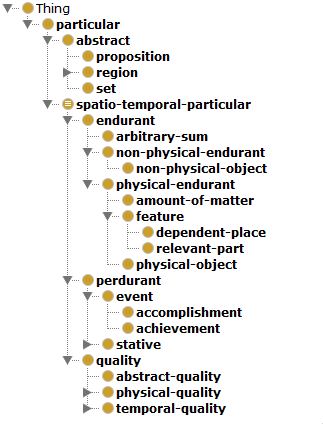
\includegraphics[width=\textwidth]{media/chapter3/dolce-taxonomy}}
\end{minipage}
\hspace{0.5cm}
\begin{minipage}[b]{0.45\linewidth}
\centering
\frame{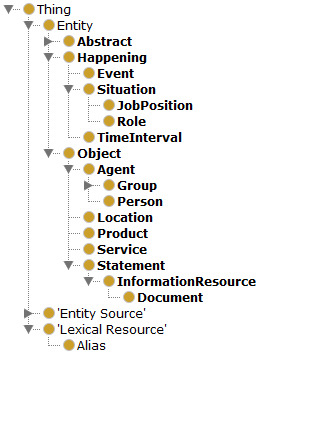
\includegraphics[width=\textwidth]{media/chapter3/proton-taxonomy}}
\end{minipage}
\caption{Dolce and Proton Class Hierarchies}
\label{fig:ontology-hierarchies}
\end{figure}

In our work, we use ontologies to model key pieces of knowledge. This includes the type of objects and relationships they are expected to have. OWL is the current standard language in authoring ontologies. The current standard being OWL 2.0. The majority of work, related to this dissertation, is in utilizing ontologies have been in the data integration domain \cite{smith2007obo, noy2004semantic, astakhov2005data}. We utilize some of the features of the declarative mapping language \cite{dou2005ontology} to express the structure of relations stored in various data sources. Specifically, we use the s-expression like syntax to declare the relations and the mapping axioms which relate items in the expression to objects in our ontology. SPARQL \cite{prud2008sparql} is the current standard for querying RDF documents. The event and entity discover queries generated by the discovery algorithm in the next chapter are generated using SPARQL templates.

We use the terminologies followed in upper level ontologies. Figure \ref{fig:ontology-hierarchies} shows the class hierarchies for the Dolce Upper Ontology (on the left) and the Proton Top Level Ontology (on the right). Similar to these taxonomies, we will use the term `entities' to collectively refer to all real-world events and objects. Events, are perdurants, and have temporal or spatial parts. Events in our context discovery will include Academic Conferences, Concerts, Photo-Capture Events or Meetings. Objects, such as Persons, on the other hand, are uniquely identifiable wholes. They do not need temporal or spatial attributes for their description. It must be noted that we extend the DOLCE-Lite upper ontology to construct our knowledge base for CueNet.

% Before looking at the different views on context, its advisable to distinguish between `objects' and `entities'. We use the word `Object' to collectively refer to events and entities. The term `object' has been used in literature to refer to things which have no temporal properties. But, in our discussion, an `object' could imply an event which exhibits temporal properties. An entity includes persons, places or organizations present in the world which do not temporal descriptors for their unique representation, for example `Starbucks, UC Irvine', `The Eiffel Tower, Paris, France', or organizations, for example `Google Inc', `Royal Society of London'. Effectively, they are objects which do not need temporal descriptors. Events, on the other hand, are objects which rely on temporal attributes.

% \begin{figure}[h]
% \centering
% 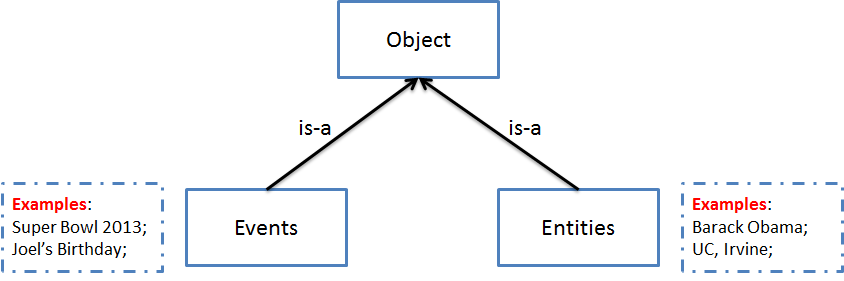
\includegraphics[width=0.6\textwidth]{media/chapter1/terminology.png}
% \caption{Objects, Events and Entities.}
% \label{fig:terminology}
% \end{figure}
